\documentclass[11pt]{article}
\setlength{\parindent}{0pt}


\usepackage{amssymb}
\usepackage{amsmath}
\usepackage{amsthm}
\usepackage{indentfirst}
\usepackage{graphicx}
\usepackage{graphicx}
\graphicspath{ {./images/} }
\pagenumbering{gobble}


\begin{document}

\section*{MA 1024 Conference 7}

\vspace{\baselineskip}
\vspace{\baselineskip}
.

\newpage


\section*{Example 1 (Triple Integral in Rectangular Coordinates, General Solids)}

Evaluate $\int \int \int_E \, xyz\, dV$, where $E$ is the solid for which $0\leq z \leq 1$, $0\leq y \leq z$, $0 \leq x \leq y$.

\newpage
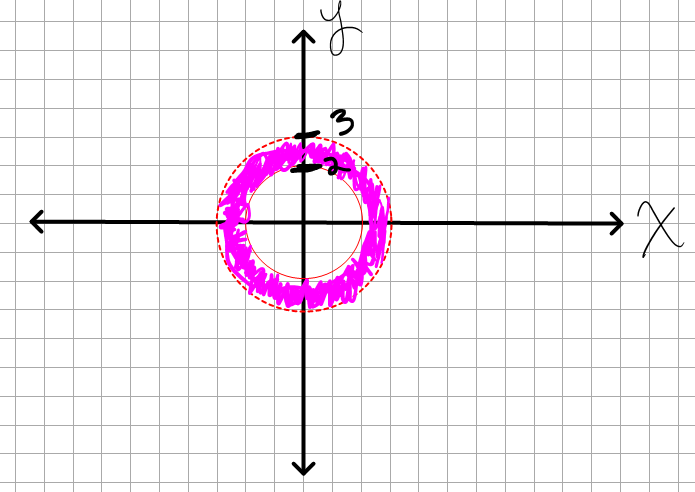
\includegraphics{Capture1.jpg}\\
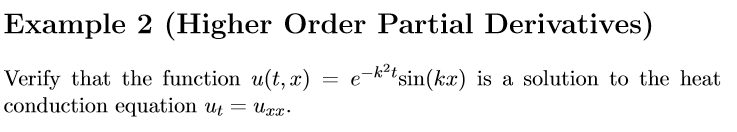
\includegraphics{Capture2.jpg}\\
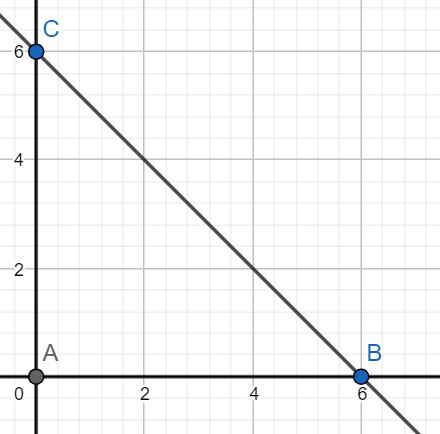
\includegraphics{Capture3.jpg}
\section*{Example 2 (Triple Integral in Rectangular Coordinates, General Solids)}

Evaluate $\int\int\int_E \, z \, dV$, where $E$ is the solid tetrahedron bounded by the four planes $x = 0$, $y = 0$, $z= 0$, and $x + y + z = 1$. \newpage

.

\newpage

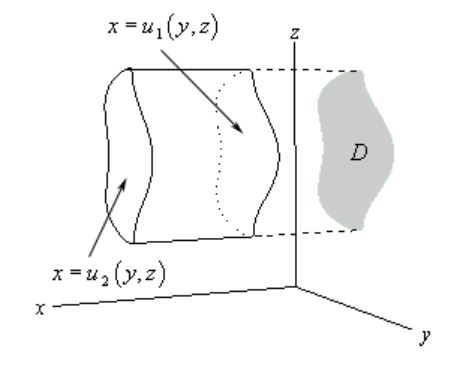
\includegraphics{Capture4.jpg}\\

\includegraphics{Capture5.jpg}\\
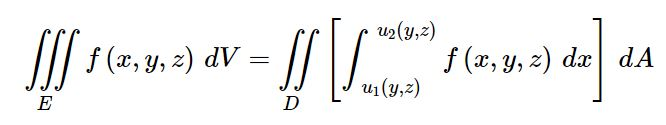
\includegraphics{Capture6.jpg}
\section*{Example 3 (Triple Integral in Rectangular Coordinates, General Solids)}


Set up the triple integral to find the mass of the tetrahedron with vertices $(0,0,0)$, $(1,1,0)$, $(1,0,0)$, and $(1,0,1)$ with the density function $\rho(x,y,z) = yx$. 

\newpage

.

\newpage


\includegraphics{Capture7.jpg}\\
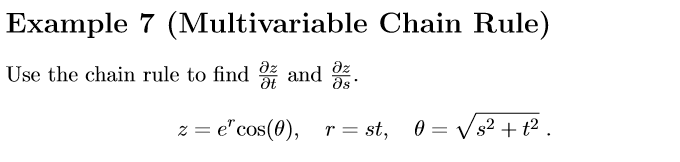
\includegraphics{Capture8.jpg}\\
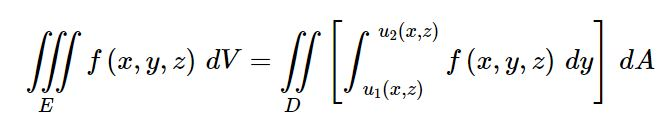
\includegraphics{Capture9.jpg}
\section*{Example 4 (Triple Integral in Rectangular Coordinates, General Solids)}
Evaluate $\int\int\int_E \, \sqrt{x^2+z^2} \, dV$, where $E$ is the region bounded by the paraboloid $y = x^2 + z^2$ and the plane $y = 4$.

\newpage
.
\newpage
\section*{Example 5 (Triple Integral in Cylindrical Coordinates)}

Evaluate $\int\int\int_E \, x^2 + y^2 \, dV$, where $E = \{(x,y,z) \; | \; -2\leq x \leq 2, -\sqrt{4-x^2} \leq y \leq \sqrt{4-x^2}, \sqrt{x^2 + y^2} \leq z \leq 2 \}$.

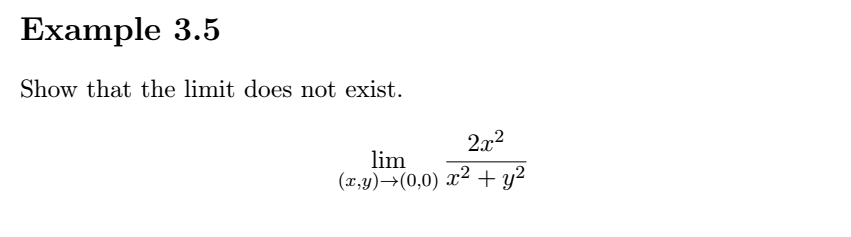
\includegraphics{Capture10.jpg}

\newpage

. 

\newpage

\section*{Example 6 (Triple Integral in Spherical Coordinates)}

Use spherical coordinates to evaluate $\int\int\int_E \frac{e^{-(x^2+y^2+z^2)}}{\sqrt{x^2+y^2+z^2}} \, dV$, where $E$ is the the hemisphere bounded by $z = \sqrt{9 - x^2 - y^2}$ and $z = 0$.

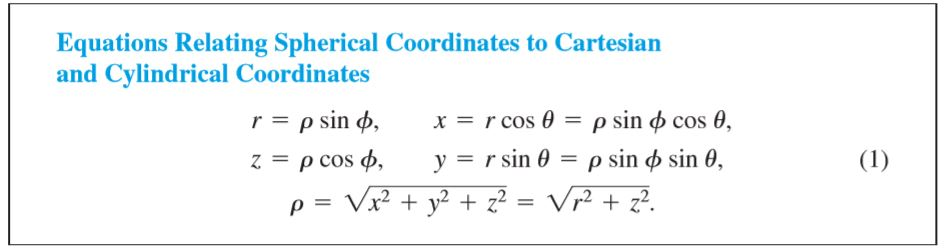
\includegraphics{Capture11.jpg}

\newpage

.

\newpage


\end{document}